\large



The study found that the GWPL was the best method to predict the PL, however the value of the surface constant was needed to be complex and therefore hard to determine. The accuracy of the PL models was found to:

\begin{center}
\begin{tabular}{|c|c|c|}
\hline
\rowcolor{white}
\textbf{Models} & \textbf{MSE} & \textbf{Applicability} \\ \hline \rowcolor{white}
FSPL            & 15.95        & 35 \%                  \\ \hline \rowcolor{white}
ATRPL 		    & 141.58       & 65 \%                  \\ \hline \rowcolor{white} %approx.
%TRPL     		& 42.12        & 100 \%                 \\ \hline
GWPL            & 35.49        & 100 \%                 \\ \hline \rowcolor{white}
NSPL            & 230.05       & 30 \%                  \\ \hline \rowcolor{white}
PPL            & 60.18        & 65 \%                  \\ \hline
\end{tabular}
\end{center}


The PPL also uses the same surface constants as the GWPL. However, only the magnitude of it is needed and it is therefore easier to find. A change in value give rise to a offset in the predicted PL.
% This file was created by matlab2tikz.
%
%The latest updates can be retrieved from
%  http://www.mathworks.com/matlabcentral/fileexchange/22022-matlab2tikz-matlab2tikz
%where you can also make suggestions and rate matlab2tikz.
%
\definecolor{mycolor1}{rgb}{0.00000,0.44700,0.74100}%
\definecolor{mycolor2}{rgb}{0.85000,0.32500,0.09800}%
\definecolor{mycolor3}{rgb}{0.92900,0.69400,0.12500}%
%
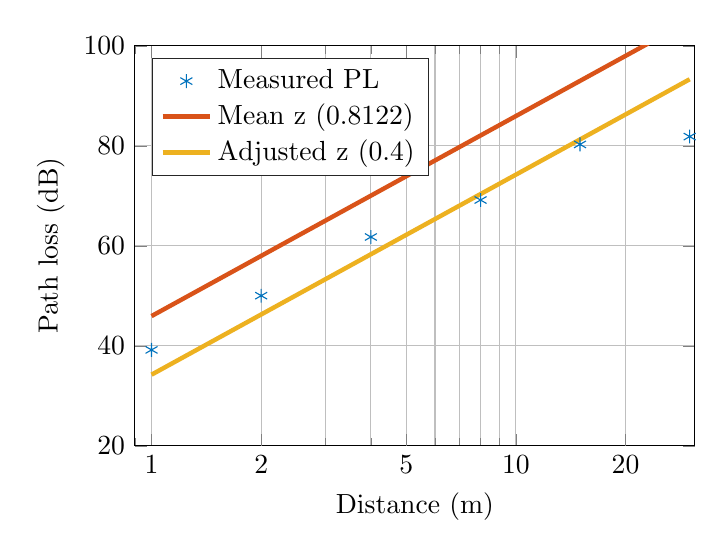
\begin{tikzpicture}

\begin{axis}[%
width=2.8in,
height=2in,
at={(2.6in,1.105in)},
scale only axis,
extra x ticks={2,5,20}, 
extra x tick style={log identify minor tick positions=false},
log ticks with fixed point,
xmode=log,
xmin=0.9,
xmax=31,
xlabel=Distance (m),
xminorticks=true,
xmajorgrids,
xminorgrids,
ymin=20,
ymax=100,
ylabel=Path loss (dB),
ymajorgrids,
axis background/.style={fill=white},
legend style={at={(0.03,0.97)},anchor=north west,legend cell align=left,align=left,draw=white!15!black}
]
\addplot [color=mycolor1,mark size=2.5pt,only marks,mark=asterisk,mark options={solid}]
  table[row sep=crcr]{%
1	39.176832441447\\
2	50.0236813268286\\
4	61.7627349006033\\
8	69.1568155321866\\
15	80.2784721484843\\
30	81.8463231335614\\
};
\addlegendentry{Measured PL};

\addplot [color=mycolor2,solid,ultra thick]
  table[row sep=crcr]{%
1	45.9420286016976\\
2	57.9832284282568\\
4	70.0244282548161\\
8	82.0656280813753\\
15	92.9856789639248\\
30	105.026878790484\\
};
\addlegendentry{Mean z (0.8122)};

\addplot [color=mycolor3,solid,ultra thick]
  table[row sep=crcr]{%
1	34.2247802230071\\
2	46.2659800495663\\
4	58.3071798761256\\
8	70.3483797026848\\
15	81.2684305852343\\
30	93.3096304117936\\
};
\addlegendentry{Adjusted z (0.4)};

\end{axis}
\end{tikzpicture}%
